\section{Servo motor}
The purpose of the servo motor is to control the "flipper", which separates the bricks. \\


A servo motor consist of a DC motor, a potentiometer and a control circuit.
As the motor rotates, the resistance of the potentiometer changes,  which the control circuit uses to regulate its movement.
When the motor is at the desired position it is blocked to avoid movement.\\


Which position the servo locks to is decided by the signal on the control wire.
The control signal resembles PWM in that it consists of periodic pulses, in fact, it can be implemented as PWM. 
It is the width of these pulses that determines the position of the motor.
See figure \ref{fig:servoposition}. Varying the pulse width between one and two ms will vary the position of the motor between 0$^\circ$ to 180$^\circ$.
 
\begin{figure}[H]
\centering
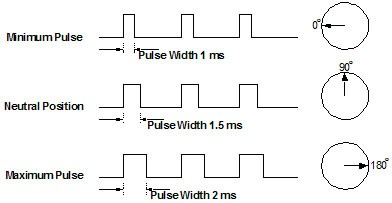
\includegraphics[scale=0.6]{images/servocontrol.jpg}
\caption{Control of a servo motor.}
\label{fig:servoposition}
%http://www.societyofrobots.com/actuators_servos.shtml
\end{figure}

\subsection{Interaction with Servo motor}
The control of the servo motor is done using the FPGA with the VHDL component named pwm. See figure \ref{fig:pwmcomp}

\begin{figure}[htb]
\centering
\begin{tikzpicture}[font=\sffamily,>=triangle 45]
  \node [shape=circuit] (item) at (0,0) {pwm};
  \draw [<-] (item.ina) node [anchor=west,labels] {} -- +(-1,0) node [anchor=east] {CLK};
  \draw [->] (item.outa) node [anchor=east,labels] {} -- +(1,0) node [anchor=west] {PWM\_motor};
  \draw [<-] (item.inb) node [anchor=west,labels] {} -- +(-1,0) node [anchor=east] {direc};
\end{tikzpicture}
\caption{Entity of pwm}
\label{fig:pwmcomp}
\end{figure}

\texttt{PWM\_motor} is connected to the control wire of the servo motor, and provides the signal that sets the position. 
\texttt{direc} is a 2 bit \texttt{std\_logic\_vector}, which tells the entity which direction the servo motor has to move in. \texttt{CLK} is the clock signal of the FPGA. \\

The component has only one process. It generates one of three different PWM signals based on the value of \texttt{direc}. 

If the value of direc is: 
\begin{itemize}
\item \textbf{"11"}: Motor moves to the right position.
\item \textbf{"00"}: Motor moves to the left position.
\item \textbf{Any other value}: Motor moves to the neutral position.
\end{itemize}


The period of the PWM signal of \texttt{PWM\_motor} is set to  20 ms, as required by the servo motor.
For each  \texttt{rising\_edge} of \texttt{CLK}, \texttt{count} is incremented.
\texttt{count} is reset at 1.000.000. This results in a period of 20ms at a frequency of 50MHz. 
To generate the PWM that will turn the motor to the leftmost position, \texttt{PWM\_motor} is set high when \texttt{count} is above 950.000 and is set low when \texttt{count} is reset. Increasing the number of rising edges where \texttt{PWM\_motor} is high will gradually move the motor towards the rightmost position generated at 100.000 rising edges.



